%!TEX root=../thesis.tex
\chapter{Real-Time background} \label{cha:rt_background}

The work described in this thesis has many theoretical foundations that has to be
clear in order to understand the reasons behind some design choiches or assumptions. 
All the needed notions in the real-time theory are explained in the following sections.


\section{Task model} \label{sec:task_model}
This model considers a set of real-time tasks \( T = \{\tau_{i}\} \)
sharing a Central Processing Unit (CPU). Every task
is composed of a stream of jobs \( J_{i,\,k} \), identifying the \( k^{th} \)
instance of the \( i^{th} \) task in the set \( T \). This concept of multiple
jobs composing a job can be better understood looking at Figure \ref{img:task_model}.
\begin{figure}[!htb]\label{img:task_model}
    \center{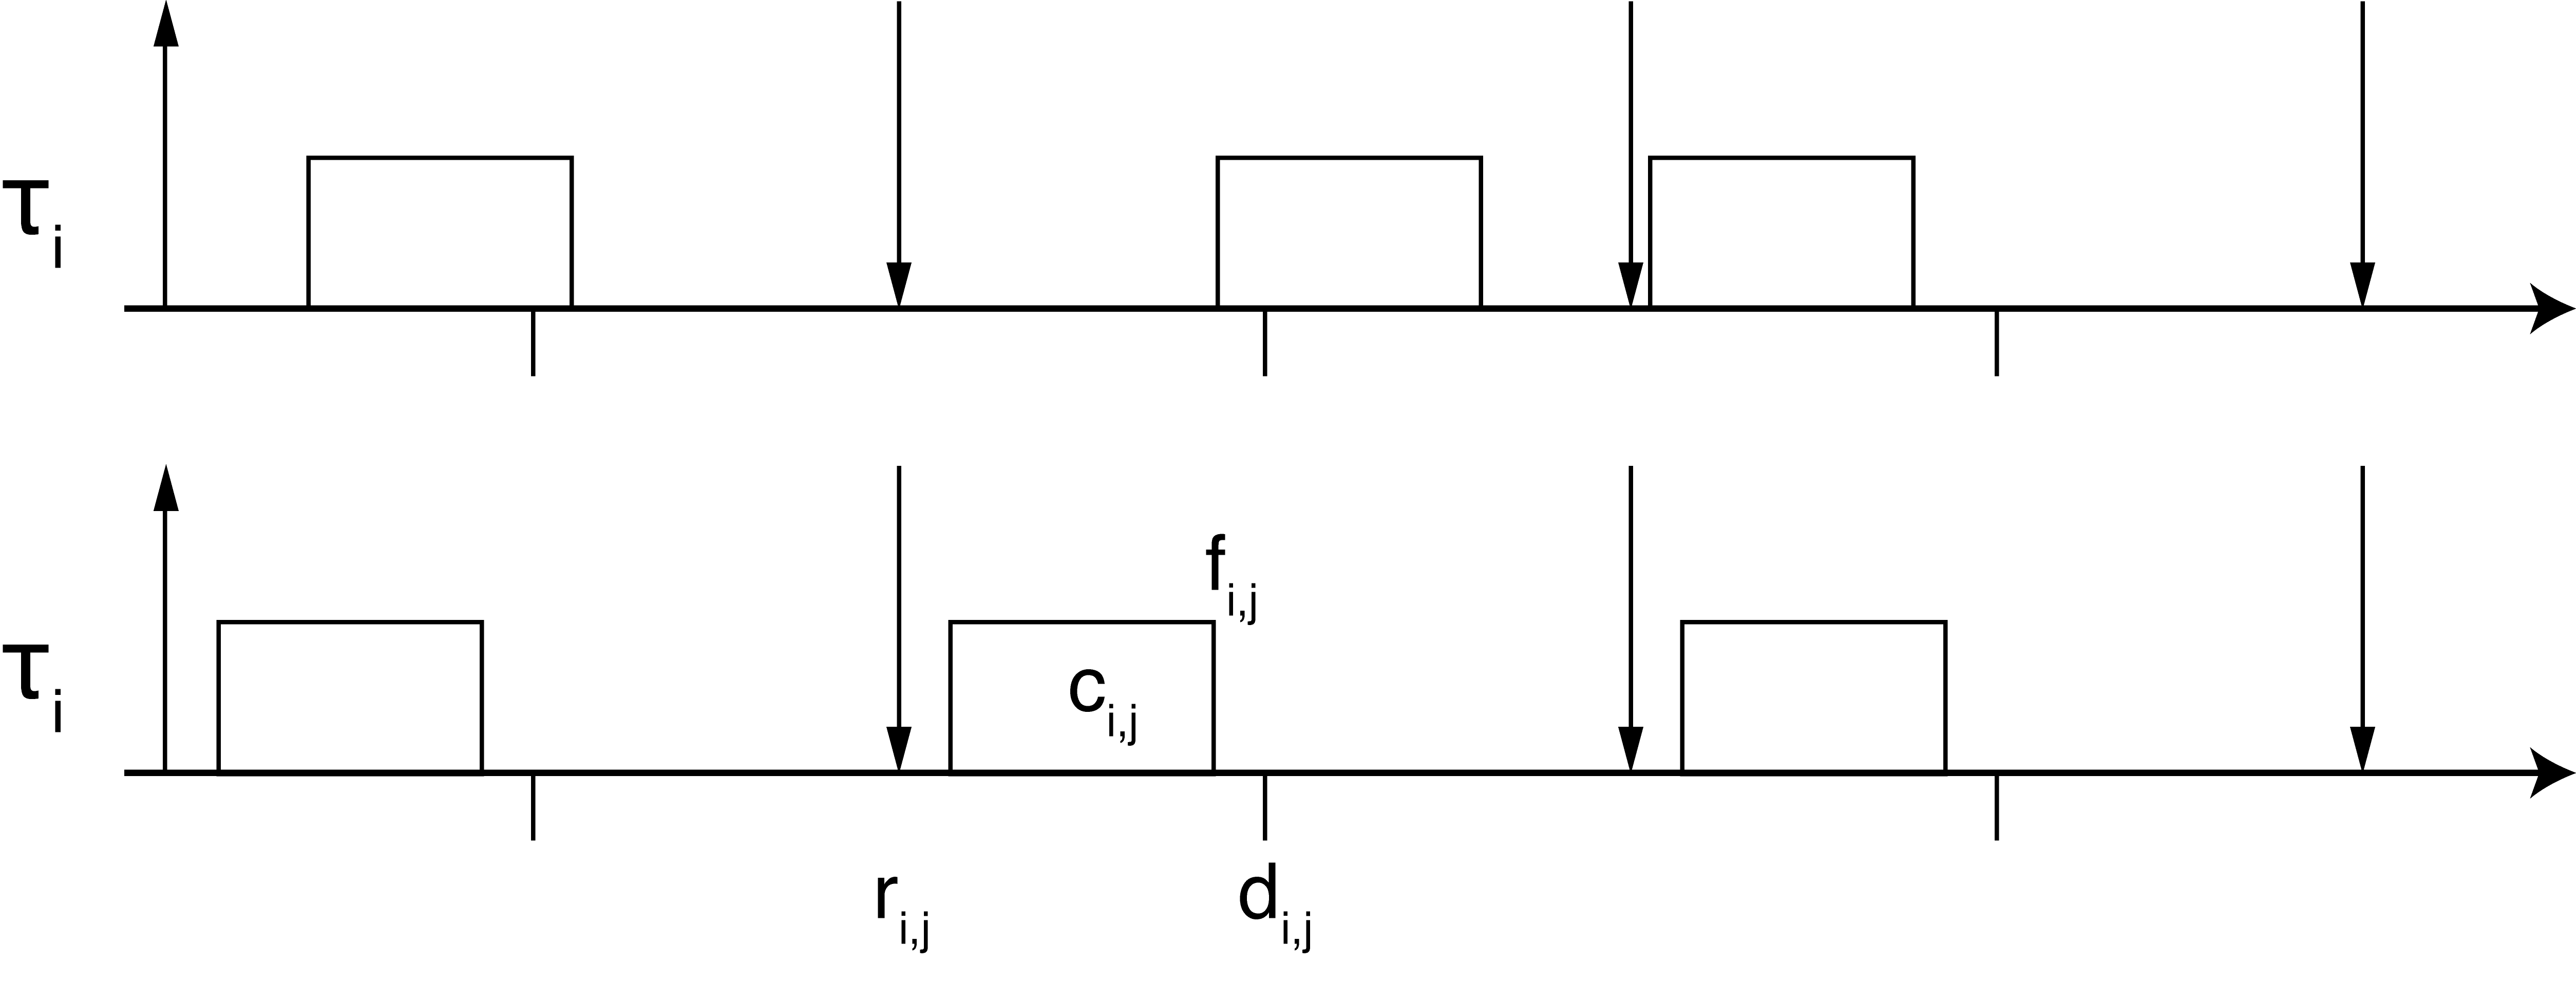
\includegraphics[width=0.7\linewidth]{task_model.png}}
    \caption{Graphical explanation of the task model.}
\end{figure}

Every job is formally defined as a touple
\( J_{i,\,k} = \left(r_{i,\,k}, \;f_{i,\,k}, \;c_{i,\,k}\right) \) where:
\begin{itemize}
    \item the indices \( i \) and \( k \) specify the number of the task and the
        instance of the job inside the task set \( T \) respectively
    \item \( r_{i,\,k} \) is the \emph{release} time; it is the time when
        the job arrives to the scheduler and it can be chosen for execution
        by the scheduler itself (and actually taken in charge by the CPU).
    \item \( f_{i,\,k} \) is the \emph{finishing} time; it is the moment when
        the computation for the job \( J_{i,\,k} \) ends.
    \item \( c_{i,\,k} \) is the \emph{computation} time, that is the amount of
        time for which the job \( J_{i,\,k} \) is running. This can also be seen
        as the real load on the CPU.
\end{itemize} 

In addition, the computation time \( c_{i,\,k} \) is generally assumed to be
independent and identically distributed (i.i.d.) stochastic process.
This happens when two random variables \( X \) and \( Y \) have 
the same probability distribution and both are mutually
independent, meaning that the occurrence of \( X \) does not \( c_{i,\,k} \) 
the probability of occurrence \( Y \) (and vice versa).
Hence for each job instance, \( c_{i,\,k} \) is a random
variable described by a certain Probability Mass Function (PMF).
The i.i.d. assumption is one of the milestones of the real-time modeling theory.
However, the analysis proposed in Chapter \ref{cha:rt_model} will relax this 
constraint following the study proposed by Fr\'{i}as, Palopoli et al
in~\cite{frias2017probabilistic}.

Another very important concept is the worst-case execution time (WCET) \( W_{i} \).
It represents the maximum fraction of CPU time spent to execute the task
\( \tau_{i} \) and it can be computed by the following equation:
\begin{equation}\label{eq:wcet}
    W_{i} = \ceil[\bigg]{\frac{c_{i,\,j}}{T_{i}}}
\end{equation}

Moreover, the total system utilization \( W_{tot} \) can be easily derived from
Equation \ref{eq:wcet} as:
\begin{equation}\label{eq:system_utilization}
    W_{tot} = \displaystyle\sum_{i} W_{i}
\end{equation}

Furthermore, every real-time job has to respect a temporal constraint called
deadline. The standard approach is to have a deterministic deadline for a job
that cannot be missed (hard real-time), but many other models handles
probabilistic deadlines (soft real-time).
More formally, every job \( J_{i,\,k} \) has a relative deadline \( D_{i} \) that
is used to define an absolute deadline \( d_{i,\,k} = r_{i,\,k} + D_{i} \).
A deadline is said to be respected if \( f_{i,\,k} \leq d_{i,\,k} \) and missed
if \( f_{i,\,k} > d_{i,\,k} \). Talking about probabilistic deadlines, it is
possible to say that a deadline is respected if 
\( \Pr\,\{f_{i,\,k} > r_{i,\,k} + D_{i} \} \leq p_{i} \) and it is missed otherwise.
The value \( p_{i} \) is the probability to meet the deadline associated
with the task \( \tau_{i} \).


\section{Different types of tasks}
Not all the tasks are equal. Thus being able to distinguish them is
very important.

The different types of tasks in the literature are \emph{periodic},
\emph{aperiodic} and \emph{sporadic}.\\
A periodic task has regular structure
and it is triggered every fixed period \( T_{i} \). Its lifetime can be seen as
a cycle, where it activates at time \( r_{i,\,k} \), it executes for an amount 
of time \( c_{i,\,k} \) and then it waits for the next period to start. The exit
condition is a characteristic of to the specific application.\\
On the contrary, as the name suggests, an aperiodic task has non-periodic arrivals.
Moreover there is no minimum inter-arrival time between the jobs and,
most of the times, these tasks do not have any recurrent structure. They are used
to model operations which occur rarely and that are irregular during the lifetime
of the application.\\
Finally, the last type is very similar to a periodic task. Both have a minimun
inter-arrival time between each activation, even though it may not be always the
same throughout the whole execution. A sporadic task is mainly triggered by an
external event (eg. a network packet) rather than using a timer as it happens
for a periodic task.


\section{Scheduler}
As it is possible to imagine, tasks do not run on bare computer hardware.
The Operating System (OS) creates the illusion that each task has a virtual CPU
where they run alone without any interference from the others.
This strategy makes them believe that they are running simultaneously on the same
machine. This statement is true if we think of a single CPU with one core. Modern
CPUs are multi-core and they give the possibility to actually run multiple tasks
at the same time. The general rule is that the number of process that can be
executed in parallel is upper-bounded by the number of available physical cores.\\
Since it is possible to run only one task at a time on a single CPU, they need
to alternate each other in order to give everyone the possibility to get their
work done. Here is where the \emph{task scheduler} starts its job: it is
responsible for scheduling a set of tasks \( \{\tau_{i}\} \). For the
sake of simplicity it is reasonable to assume that a CPU has only one core.

There exist several scheduling algorithms that can be used to select, at every
instant \emph{t}, which is the task to be executed. More in general, it is
possible to say that a scheduling algorithm \emph{A} generates a schedule
\( \sigma_{A}\left(t\right) \) starting from a set of tasks \( T = \{\tau_{i}\} \).\\
Furthermore, a schedulability test can be performed to see if the scheduling
algorithm \( A \) is able to schedule a given task set \( T \). This checks
if the schedule \( \sigma_{A}\left(t\right) \) generated by the algorithm \emph{A}
guarantees that every deadline (probabilistic or not) is never missed.
Some of the most famous scheduling algorithms in the computer science literature
are Rate Monotonic (RM)~\cite{lehoczky1989rate}, Deadline Monotonic
(DM)~\cite{audsley1991hard} and Earliest Deadline First (EDF)~\cite{jansen2003lightweight}.
Another well known approach is the \emph{sched\_deadline}~\cite{lelli2016deadline}
algorithm, which is used in the Linux kernel as default scheduling algorithm from
the 3.14 version.


\section{Resource Reservation scheduling}
Since multiple real-time tasks can run concurrently on the same CPU, there
exist another possible approach. The resource reservation 
(RR)~\cite{abeni1998integrating} algorithm allows to associate to each task 
\( \tau_{i} \) a reservation \( \left(Q_{i}^s, T_{i}^s\right) \). 
The RR algorithm allows the \( i^{th} \) task to only run for \( Q_{i}^s \) time units 
in every interval of length \( T_{i}^s \). The value \( Q_{i}^s \) is defined as
\emph{budget}, while \( T_{i}^s \) is known as the \emph{reservation period}.
This approach allows to allocate a fraction of CPU time for a task \( \tau_{i} \)
called \emph{bandwidth} and it is calculated as follows:
\begin{equation}
    B_{i} = \frac{Q_{i}^s}{T_{i}^s}
\end{equation}

In this way the scheduler reserves for each task an amount of computation
time \( Q_{i}^s \) in each reservation period \( T_{i}^s \). This constraint
prevents tasks to run for more time than the selected budget and
therefore each task does not need to take into account the other operations running
concurrently on the CPU. This very important property for RR algorithm is called
\textbf{temporal isolation} and it is valid as long as the scheduling
condition~\cite{lee2007handbook} shown in Equation \ref{eq:temporal_isolation} 
holds. This property allows the system and application designer to analyze every
task on its own, making its life much easier.

\begin{equation} \label{eq:temporal_isolation}
    \displaystyle\sum_{i} B_{i} =  \displaystyle\sum_{i} \frac{Q_{i}^s}{T_{i}^s} \leq 1
\end{equation}


\section{Hard vs. soft real-time}
As previously mentioned in Section \ref{sec:task_model}, there exist two different
notions of real-time.

In hard real-time systems every deadline for a job must be respected, meaning
that even a single dealine miss implies a system failure. This is the case, for
example, of some medical applications like pacemakers and some avionics systems.
The requirements for soft real-time systems are looser.\\
On the other hand, a soft real-time application is allowed to miss some deadline,
degradating the performance and the quality of the service.
This is what happens in straming video players for example, where missing the
deadline for some frame may not even noticed by the user. Clearly, if too many
frames are not displayed on the screen, the streaming cannot be enjoyed by the
user in any way. Another notheworthy aspect is that if a soft real-time system
misses some deadline no critical failure happens and no life is put in danger.
Obviously this is clearly not the case for the other ones, where a potential
disaster happens only due to a single deadline miss of the entire system.\\
Focusing on the work of this thesis, the 3D navigator developed to study how
real-time models can be applied to web technologies and, more specifically, to
WebGL. This case study is obviously a case of soft real-time application, since
no life is put in danger and no critical system fails because of this part of
of the FriWalk architechture.
